% Source of 043_report_extended_zh.pdf. Build in this folder with two runs of
%   xelatex -jobname=043_report_extended_zh main.tex
% (fonts: TeX Gyre Termes/Heros, STIX Two Math, Noto Serif CJK SC) and copy 043_report_extended_zh.pdf to ../
\documentclass[a4paper,11pt]{article}
\usepackage{fontspec}
\setmainfont{TeX Gyre Termes}
\setsansfont{TeX Gyre Heros}
\newfontfamily\cjkfont{Noto Serif CJK SC}
\usepackage{amsmath}
\usepackage{unicode-math}
\setmathfont{STIXTwoMath-Regular.otf}
\usepackage[a4paper,top=2.5cm,bottom=2.4cm,left=2.6cm,right=2.6cm]{geometry}
\usepackage{graphicx,booktabs,array,threeparttable,pdfpages,fancyhdr,xurl}
\usepackage[font=small,labelsep=period,skip=4pt]{caption}
\usepackage[hidelinks,bookmarksnumbered=true,bookmarksopen=true]{hyperref}
\usepackage{titlesec}
\renewcommand{\floatpagefraction}{0.8}\renewcommand{\topfraction}{0.88}\renewcommand{\bottomfraction}{0.7}\renewcommand{\textfraction}{0.1}
\usepackage{etoolbox}\AtBeginEnvironment{thebibliography}{\small\linespread{1.05}\selectfont\setlength{\itemsep}{1pt}\setlength{\parskip}{0pt}}
\setlength{\emergencystretch}{3em}
\linespread{1.15}
\setlength{\parskip}{0.25em}
\titleformat{\section}{\large\bfseries}{E\arabic{section}}{0.8em}{}
\titleformat{\subsection}{\normalsize\bfseries}{E\arabic{section}.\arabic{subsection}}{0.6em}{}
\renewcommand{\thesection}{E\arabic{section}}
\renewcommand{\thefigure}{E\arabic{figure}}
\renewcommand{\thetable}{E\arabic{table}}
\renewcommand{\theequation}{E\arabic{equation}}
\setlength{\headheight}{15pt}\pagestyle{fancy}\fancyhf{}\renewcommand{\headrulewidth}{0.4pt}
\newcommand{\hd}[1]{\begin{tabular}[b]{@{}c@{}}#1\end{tabular}}
\newcommand{\exthead}[1]{\fancyhead[L]{\small #1}\fancyhead[R]{\small Part II\quad Post-competition extensions}\fancyfoot[C]{\small E-\thepage}}

\graphicspath{{../../figures/extension/}}
\hypersetup{pdftitle={Stable credit scores after a limit increase -- extended edition}}
\begin{document}
\thispagestyle{empty}
\begin{center}
{\Large\bfseries Stable Credit Scores after a Limit Increase:\\[0.2em] Reference Scale, Near-Stable Updates and Capacity Protection}\\[0.7em]
{\large Extended edition --- note}
\end{center}
\vspace{0.8em}

This file has two parts. Part I is the report submitted to Task 1 of the data-analysis track of the 2026 FinTechathon, the Shenzhen International Fintech Competition (28 pages, in Chinese), reproduced exactly as submitted. Part II, starting on page E-1, contains post-competition extensions written in November 2026.

The final score proposed in the report has three parts: a base model on a reference scale, near-stable updates that keep customers who pass a stability gate within $\pm1$ percentage point of their previous score, and capacity protection that restores the review list of the base model. Part II tests two of these design choices that the report did not justify. E1 shows that the separating threshold of the capacity protection is a free parameter. The midpoint rule of the report changes the fewest scores, the exact L2-minimal rule touches five times as many customers, and a rule that minimises broken stability promises lowers their number from 14 to 11, all with identical AUC. E2 compares stabilisation variants in exactly the same period-by-period replay. The radius of $\pm1$ percentage point lies on a flat stretch, whereas dropping the gate and clipping every update at $\pm2$ percentage points keeps the AUC and lowers the tail instability of the worst cohort by 39\,\%.

Part II publishes only aggregate results; row-level customer data are not distributed with the repository. Every number can be reproduced from the original inputs with the scripts in the \texttt{extension/} folder of the code repository; result files are in \texttt{results/extension/}.

\clearpage
\pdfbookmark[0]{Part I\quad Competition report (as submitted)}{part1}

\includepdf[pages=-]{../../package/043-赛题1.pdf}
\pdfbookmark[0]{Part II\quad Post-competition extensions}{part2}
\setcounter{page}{1}
\exthead{Stable credit scores after a limit increase}
\begin{center}{\Large\bfseries Part II\quad Post-competition extensions}\end{center}

The report addresses non-risk-driven score fluctuation after a credit-limit increase and builds a final score on the public Home Credit data\cite{homecredit}. In the limit-increase month its AUC is 0.8171 on 2\,907 customers; the 559 review slots of the two periods cover 61 customers who become early delinquent within three months; and among customers with similar states the most extreme 5\,\% of score changes are 39.5--68.8\,\% smaller than those of a strong risk ensemble. The final score contains two design choices that the report does not justify on their own: the separating threshold of the capacity protection, and applying the $\pm1$ percentage point limit only to customers who pass the stability gate. The two extensions below test these choices, and every comparison uses exactly the same period-by-period replay as the submission.

\section{Which separating threshold should capacity protection use?}

\subsection{Formulation}
Capacity protection clips the stabilised candidate scores $z$ at a threshold $\tau$ so that the protected set, the top $k$ customers of the base model, stays unchanged; the submission places $\tau$ at the midpoint between the $k$-th and the $(k+1)$-th base score. Any $\tau$ that separates the protected set from the other customers is admissible, so the threshold is a free design parameter. For a fixed $\tau$, the closest admissible score is $f_i=\max(z_i,\tau^+)$ for a protected customer and $f_j=\min(z_j,\tau)$ for an unprotected one, and the total squared change
\begin{equation}
C(\tau)=\sum_{i\in P}(\tau-z_i)_+^2+\sum_{j\in U}(z_j-\tau)_+^2
\end{equation}
is convex in $\tau$ with a monotone derivative, so the exact L2-minimal threshold can be found by bisection. A second rule minimises, in lexicographic order, the number of gated customers pushed outside their $\pm1$ percentage point stability promise, the total excess, and the total change. All three rules are replayed in exactly the same period-by-period pipeline (same phases, cross-fitting folds, gate, radius 0.01 and 10\,\% review capacity).

\subsection{Results}
\begin{table}[htbp]\centering\small\setlength{\tabcolsep}{4pt}
\caption{Three rules for the separating threshold (5\,584 updates; ``broken promises'' counts gated customers whose score moves outside $\pm1$ percentage point, ``total excess'' sums the part outside).}\label{tab:ft-e1}
\begin{tabular}{lrrrrr}\toprule
Separating threshold & \hd{Scores\\changed} & \hd{Broken\\promises} & \hd{Total\\excess} & \hd{L2\\change} & \hd{AUC\\(limit month)}\\\midrule
Midpoint of base scores (submitted) & \textbf{14} & 14 & \textbf{25.7 pp} & 0.191 & 0.8171\\
Exact L2-minimal change & 68 & 19 & 30.0 pp & \textbf{0.187} & 0.8171\\
Fewest broken stability promises & 54 & \textbf{11} & 28.4 pp & 0.200 & 0.8171\\\bottomrule
\end{tabular}
\end{table}

\begin{figure}[htbp]\centering
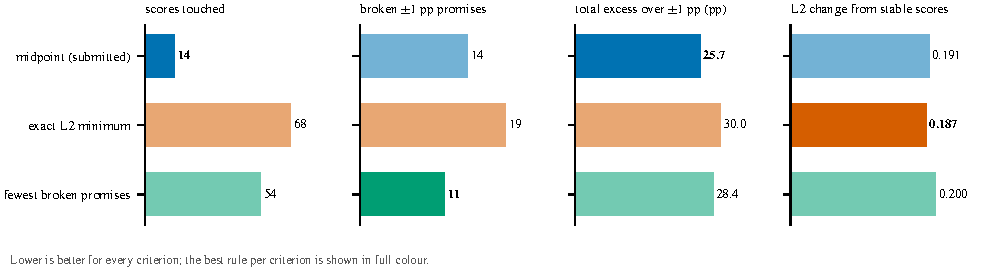
\includegraphics[width=0.6\textwidth]{figE1_guard_threshold_tradeoff.pdf}
\caption{Trade-off between the number of scores changed and broken stability promises under the three threshold rules.}\label{fig:ft-e1}
\end{figure}

No rule dominates (Table~\ref{tab:ft-e1}, Figure~\ref{fig:ft-e1}). The submission's ``minimal change'' holds in the operational sense, since it changes the fewest scores and adds the least excess, but not in the L2 sense: the exact L2 projection spreads small changes over five times as many customers. If the business promise concerns the number of customers whose score leaves the $\pm1$ percentage point band, another threshold lowers the broken promises from 14 to 11 ($-21\,\%$), at the price of small adjustments to 40 further customers outside the gate. Discrimination is unaffected by the choice (the AUC is identical to four decimal places), and the top-10\,\% review lists are identical by construction. The threshold is therefore purely a matter of operating policy and can be exposed to the business as a parameter of the scorer.

\section{Is the stability gate necessary, and is \texorpdfstring{$\pm1$}{±1} percentage point the right radius?}

\subsection{Design}
The final score contains two further design choices: a customer's score is held within 1 percentage point of the previous period's score, and only when the account's transaction flow passes the stability gate. The usual practice in the literature on prediction churn is instead to clip or exponentially smooth every update without a gate\cite{fard2016,jiang2022}. E2 places these variants in exactly the same period-by-period pipeline: the same phases, out-of-fold batches, 10\,\% slots per fold and capacity protection. Every variant built on the same base model therefore reviews exactly the same customers as that base model, and only stability and discrimination change. The parameterised replay reproduces the published final score exactly (largest absolute difference 0).

Tail instability is measured as in the report, by the mean of the largest 5\,\% of absolute score changes (CVaR$_{95}$\cite{rockafellar2000}), and the worst value is taken over three cohorts whose risk has not changed (stable customers who pass the gate, customers with a similar repayment state, customers with a similar payment structure) and over both months. Paired intervals come from a customer-level bootstrap with 1\,000 resamples.

\subsection{Results}
\begin{table}[htbp]\centering\footnotesize\setlength{\tabcolsep}{4pt}
\caption{Comparison of stabilisation variants (reference-scale base model; the last two columns give the difference from the submission with 95\,\% paired bootstrap intervals).}\label{tab:ft-e2}
\begin{tabular}{lcccc}\toprule
Variant & \hd{AUC,\\two months} & \hd{Worst-cohort\\CVaR$_{95}$ (pp)} & $\Delta$AUC & $\Delta$CVaR$_{95}$ (pp)\\\midrule
No stabilisation & 0.7956 & 7.38 & --- & ---\\
\textbf{Submitted: gate + $\pm1$ pp} & 0.7953 & 5.29 & --- & ---\\
Gate + $\pm0.25$ to $\pm2$ pp & 0.7949--0.7955 & 5.29--5.30 & --- & ---\\
Clip every update at $\pm2$ pp & 0.7953 & \textbf{3.25} & $[-0.0020, +0.0026]$ & $[-3.33, -1.08]$\\
Clip every update at $\pm1$ pp & 0.7928 & 2.54 & $[-0.0080, +0.0023]$ & $[-4.03, -1.75]$\\
Smooth every update, weight 0.75 & 0.7857 & 3.06 & --- & ---\\\bottomrule
\end{tabular}
\end{table}

\begin{figure}[htbp]\centering
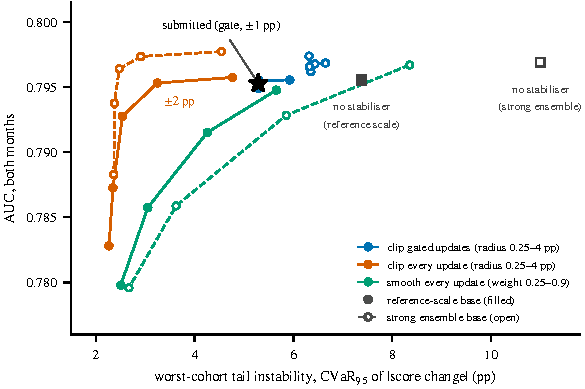
\includegraphics[width=0.47\textwidth]{figE2_stability_frontier.pdf}
\caption{AUC against worst-cohort tail instability. Lines sweep the clipping radius or the smoothing weight; filled markers use the submission's reference-scale base model, open markers the strong risk ensemble.}\label{fig:ft-e2}
\end{figure}

The radius lies on a flat stretch (Table~\ref{tab:ft-e2}): between 0.25 and 2 percentage points the tail instability of the worst cohort hardly changes. That cohort is the customers with a similar repayment state in the limit-increase month, and the gate covers only 38\,\% of their 1\,063 score changes, so their tail comes from customers outside the gate. Dropping the gate does move the frontier (Figure~\ref{fig:ft-e2}): clipping every update at $\pm2$ percentage points leaves the AUC unchanged and lowers the worst-cohort tail instability by 39\,\% (from 5.29 to 3.25 percentage points, an interval that excludes zero). Exponential smoothing, the distillation-style alternative, is dominated by clipping: the same tail stability costs more AUC.

The report's comparison with the strong risk ensemble holds: without stabilisation the ensemble is far less stable (CVaR$_{95}$ of 10.99 percentage points; 95\,\% bootstrap interval of the difference to the submission $[+2.9, +8.2]$ percentage points). With the same clipping of every update at $\pm2$ percentage points, however, it reaches an AUC of 0.7974 and a CVaR$_{95}$ of 2.91 percentage points (reference-scale base model: 0.7953 and 3.25). Against the submission, the 95\,\% interval of its tail difference is $[-3.9, -1.0]$ percentage points, and the interval of its AUC difference, $(-0.006, +0.010)$, includes zero; its review lists cover one fewer delinquent customer (60 against 61). Much of the stability therefore comes from the stabiliser rather than from the reference scale.

What the gate is for cannot be tested with the available labels. The gate exists so that customers whose risk genuinely changes are not held back, but in this sample even the unstabilised base model does not raise the scores of customers who later become early delinquent in the limit-increase month (mean change $-0.30$ percentage points, share of increases 46\,\%).

\subsection{Conclusions and limits}
The case for the gate can therefore rest only on design arguments. On the evidence of this section, clipping every update at $\pm2$ percentage points can serve as the default operating policy, with the gate kept as an option. All comparisons rest on the same public data and the same replay pipeline, the delinquency labels cover only three months, and the protection the gate offers to customers whose risk really changes can be assessed only with a longer observation period or more real risk events.

\begin{thebibliography}{9}
\bibitem{homecredit} Home Credit Group. Home Credit Default Risk. Kaggle competition, 2018. \url{https://www.kaggle.com/c/home-credit-default-risk}.
\bibitem{fard2016} M. M. Fard, Q. Cormier, K. Canini, M. Gupta. Launch and iterate: Reducing prediction churn. In \emph{Advances in Neural Information Processing Systems 29}, 2016.
\bibitem{jiang2022} H. Jiang, H. Narasimhan, D. Bahri, A. Cotter, A. Rostamizadeh. Churn reduction via distillation. In \emph{International Conference on Learning Representations}, 2022.
\bibitem{rockafellar2000} R. T. Rockafellar, S. Uryasev. Optimization of conditional value-at-risk. \emph{Journal of Risk}, 2(3): 21--41, 2000.
\end{thebibliography}
\end{document}
